\section{Metaheurística GRASP}
	\subsection{Desarrollo}
Hemos propuesto dos métodos que computan una solución, formulándola en base a criterios heurísticos. La limitación de los enfoques anteriores reside en que se recorre el espacio de soluciones hasta que no es posible mejorar la solución. Como sabemos que una solución maximal no necesariamente es máxima, sería útil poder contrastar distintas soluciones maximales y elegir la mejor. En otras palabras, quisiéramos ramificar la exploración del espacio de soluciones, para así aumentar nuestras posibilidades de encontrar la clique de máxima frontera.

Habiendo notado que heurísticas determinísticas siempre toman la misma decisión en el mismo paso, se propone la utilización de una heurística pseudo-greedy. Esta heurística aleatoriamente tomará decisiones localmente buenas pero no necesariamente óptimas. Se considerará que la decisión de agregar un nodo es buena si agregarlo aumenta el tamaño de la frontera. Para tener cierto control sobre que tan goloso es el comportamiento de esta heurística, se puede pedir que la elección aleatoria sea tomada teniendo en cuenta solo el mejor porcentaje de las decisiones posibles (es decir, que se elija aleatoriamente una opción buena dentro del X por ciento más alto). Si el porcentaje es chico, solo se consideraran las mejores opciones y el comportamiento será muy similar a la heurística greedy pura. Esto restringiría la ramificación que buscabamos. Si el porcentaje es muy alto, existirá la posibilidad de agregar un nodo de grado muy bajo a la clique, lo cual restringirá en gran medida la cantidad de nodos que se pueden agregar, obteniendo muy posiblemente una clique pequeña. 


\begin{algorithm}[H]
	\NoCaptionOfAlgo
	\caption{\algoritmo{randomGreedy}{\In{listaAdyacencia}{lista}, \In{float}{porcentajeConsiderado}}{clique}}
	
	nodosConsiderados $\leftarrow$ nodos(lista)
	
	ordenarPorGrado(nodosConsiderados)
	
	indiceNodoAleatorio $\leftarrow$ nodoAleatorio(nodosConsiderados, porcentajeConsiderado)
	
	nodoPorAgregar $\leftarrow$ nodosConsiderados[indiceNodoAleatorio]
	
	agregarNodoAClique(res, nodoPorAgregar)
	
	nodosConsiderados $\leftarrow$ nodoPorAgregar.adyacentes()

	ordenarPorGrado(nodosConsiderados)
	
	res $\leftarrow$ recurRandomGreedy(lista, res, nodosConsiderados, porcentajeConsiderado)


\end{algorithm}

\begin{algorithm}[H]
	\NoCaptionOfAlgo
	\caption{\algoritmo{recurRandomGreedy}{\In{listaAdyacencia}{lista}, \In{clique}{cliqueParcial}, \In{listaNodos}{nodosConsiderados}\In{float}{porcentajeConsiderado}}{clique}}
	
	\If{nodosConsiderados.size() $=$ 0}
	{
		return cliqueParcial
	}
	
	\For{nodo $\in$ nodosConsiderados}
	{
		\If{nodo.grado() $<$ cliqueParcial.size() * 2 $\vee$ nodo.esAdyacenteATodos(clique, lista)}
		{
			nodosConsiderados.borrar(nodo)
		}
	}

	\If{nodosConsiderados.size() $=$ 0}
	{
		return cliqueParcial
	}
	
	indiceNodoAleatorio $\leftarrow$ nodoAleatorio(nodosConsiderados, porcentajeConsiderado)
	
	nodoPorAgregar $\leftarrow$ nodosConsiderados[indiceNodoAleatorio]
	
	agregarNodoAClique(res, nodoPorAgregar)

	nodosConsiderados.borrar(nodoPorAgregar)
	
	res $\leftarrow$ recurRandomGreedy(lista, cliqueParcial, nodosConsiderados, porcentajeConsiderado)

\end{algorithm}

\begin{algorithm}[H]
	\NoCaptionOfAlgo
	\caption{\algoritmo{nodoAleatorio}{\In{listaNodos}{nodosConsiderados}\In{float}{porcentajeConsiderado}}{clique}}
	
		cantidadPorConsiderar $\leftarrow$ nodosConsiderados.size() $*$ (1 - porcentajeConsiderado)
		
		res $\leftarrow$ random(rango(cantidadPorConsiderar))

\end{algorithm}

Cada vez que se elige un nodo, se hace eligiendo aleatoriamente uno que esté entre los mejores de la lista de nodos agregables. En un principio, todos los nodos son elegibles para formar una clique trivial de tamaño uno. El criterio utilizado para elegir alguno es la priorización de nodos de grado alto. Es por esto que en primer lugar se ordenan los nodos en base a su grado y, luego, se elige uno aleatoriamente entre los primeros. El porcentaje a considerar es una variable de entrada que determinará el comportamiento de la heurística.

La función recursiva tiene un procesamiento muy similar, pero toma como parámetro a una clique y una lista de nodos a considerar. En el caso base, si no quedan nodos por considerar, la clique es maximal. Sino, toma la lista y le filtra los nodos que no son adyacentes a todos los nodos de la clique o que no agrandarían la frontera por tener un grado muy chico. Vuelve a preguntar si quedan nodos a considerar y, en caso afirmativo, elige un nodo aleatorio entre los mejores y lo agrega a la clique. Elimina a ese nodo de la lista de nodos a considerar y se llama recursivamente. Como en cada paso la cantidad de nodos a considerar disminuye al menos en una unidad, sabemos que la función eventualmente llega al caso base.

La metaheurística GRASP utiliza tanto búsqueda local como greedy aleatorio. La idea esta en que greedy aleatorio avanza estocásticamente por el espacio de soluciones hasta que llega a una solución maximal. Posteriormente esta solución se pasa como parametro a la búsqueda local. Si hacemos esto muchas veces, tenemos la posibilidad de llegar a muchas soluciones diferentes y así quedarnos con la mejor. Se memoriza la mejor encontrada y en cada iteración del ciclo se compara una nueva solución. Si iteramos lo suficiente, tendremos seguridad de que la solución que guardamos es la mejor entre muchas posibilidades. 

\begin{algorithm}[H]
	\NoCaptionOfAlgo
	\caption{\algoritmo{grasp}{\In{listaAdyacencia}{lista}, \In{unsigned int}{iteraciones}, \In{float}{porcentajeConsiderado}}{clique}}

	bestClique $\leftarrow \emptyset$
	 
	\For{i $\in$ rango(iteraciones)}
	{
		tempClique $\leftarrow$ local(randomGreedy(lista, porcentajeConsiderado))
		 
 		\If{bestClique.frontera() $<$ tempClique.frontera()}
		{
			bestClique $\leftarrow$ tempClique
		}
		 
	}
	
	res $\leftarrow$ bestClique

\end{algorithm}

\subsection{Cota temporal}
La complejidad de randomGreedy está dada por:

\begin{itemize}
    \item \textbf{nodos(lista)}: Devuelve una lista que contiene a todos los nodos del grafo en $O(n)$.

	\item \textbf{ordenarPorGrado}: Esta función utiliza por detrás el sort de la STD, y como lo usamos para ordenar toda la lista de nodos, su complejidad en peor caso es de $O(n*log(n))$.

	\item \textbf{indiceNodoAleatorio}: Devuelve un número aleatorio en $O(1)$.

	\item \textbf{agregarNodoAClique}: Se encarga de actualizar la clique agregando atrás del vector de nodos en la clique el nodo a insertar en $O(1)$.	

\end{itemize}

Con estos costos analizados, y considerando que la función \textbf{esAdyacenteATodos} fue analizada en casos anteriores, podemos pasar a analizar la complejidad de la función recursiva. Dado que esta función termina cuando el parámetro nodosPorConsiderar es de tamaño cero, y que en el peor de los casos puede empezar siendo de tamaño $O(n)$ y decrecer en una unidad en cada llamada recursiva, se concluye que en el peor de los casos se realizarán $O(n)$ llamadas recursivas. En cada una, hay un ciclo de $O(nodosPorConsiderar)$ iteraciones, donde por dentro se llama a la funcion \textbf{esAdyacenteATodos}, que es $O(n)$. Como en el peor de los casos nodosPorConsiderar decrece de a una unidad, la complejidad se reduce a considerar las $n$ llamadas recursivas, que cuentan dentro con un ciclo de $n$ nodos y un algoritmo de complejidad $O(n)$. Por lo tanto, nuestra complejidad acaba siendo $O(n^3)$.

Dado que GRASP esta compuesto por un ciclo que corre tantas veces como se le especifique en el parámetro iteraciones, el costo temporal va a depender linealmente del número de iteraciones. Por otro lado, hay que considerar que en cada iteración del ciclo se realiza una llamada a localSearch(randomGreedy()). Por lo tanto, lo que acaba ocurriendo es que se suman las complejidades de ambos algoritmos (pues Local Search corre solo una vez sobre la clique generada, por lo que su complejidad es ajena a la de randomGreedy). Por ende, el costo de localSearch(randomGreedy()) es $O(n^3)$ + $O((min(n,m))^3$ $\times$ $n^2)$, y como no podemos afirmar nada sobre $min(n,m)$, no podemos realizar ninguna cota. Por lo tanto, nuestra complejidad acaba siendo $O(n^3 + min(n,m))^3$ $\times$ $n^2)$.

\subsection{Casos Patológicos}

Ya que la metaheurística tiene un grado de aleatoriedad, es difícil encontrar casos patológicos. Sin embargo, como la misma utiliza internamente las heurísticas de búsqueda local y constructiva golosa, cuyo casos patológicos son parecidos, tendremos en cuenta este tipo de instancias. De cualquier manera, hay que ganarle a la probabilidad que se seleccione algún nodo de los de la clique de la mejor solución. Para evitarlo, hay que disminuir la probabilidad de que seleccione uno de estos nodos, por lo que podemos generar muchas componentes como la de mayor grado para que sea muy probable que, en las iteraciones, seleccione estos nodos en vez de los de la solución máxima. Notemos que podemos generar la cantidad que queramos de este tipo de componentes por lo que mientras más generemos, menos probabilidad tendremos de seleccionar la clique.
\subsection{Experimentación}

Al experimentar con la metaheurística, primero decidimos analizar el impacto lineal de las iteraciones:

\noindent
\begin{minipage}{0.55\textwidth}
    \hfill
    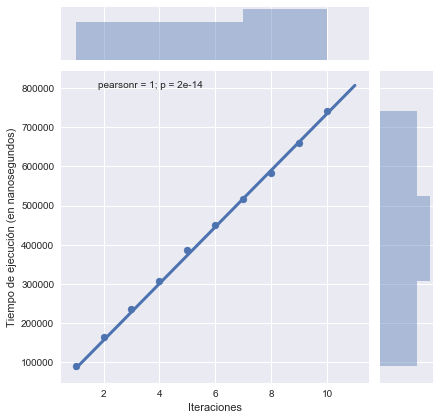
\includegraphics[scale=0.6]{img/grasp-it.png}
\end{minipage}
\hfill
\begin{minipage}{0.44\textwidth}
    \begin{center}
        Datos del gráfico

        \begin{tabular}{ | l l |}
            \hline
             & $n = 10$ \\ 
             & $m = 20$ \\ 
            Porcentaje de nodos & \\
            considerados & $p = 0.5$ \\ 
            Curva aproximada & $f(x) = 72500 * x * 10000$ \\
            \hline
        \end{tabular}
    \end{center}
\end{minipage}

Este resultado era más que esperado, ya que resulta de ejecutar las mismas operaciones una cantidad fija de veces. Teniendo esto en cuenta, podemos analizar los demás factores en el caso de una única iteración.

\noindent
\begin{minipage}{0.55\textwidth}
    \hfill
    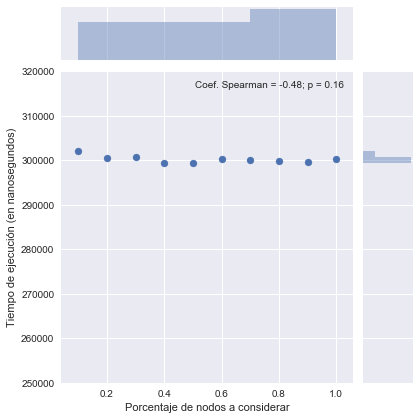
\includegraphics[scale=0.6]{img/grasp-p.png}
\end{minipage}
\hfill
\begin{minipage}{0.44\textwidth}
    \begin{center}
        Datos del gráfico

        \begin{tabular}{ | l l |}
            \hline
             & $n = 10$ \\ 
             & $m = 20$ \\ 
            Iteraciones & $it = 1$ \\
            \hline
        \end{tabular}
    \end{center}
\end{minipage}

Por el otro lado, el porcentaje de nodos del grafo a considerar se comporta de manera muy peculiar con respecto a la complejidad. Procedimos a analizar más casos para comprender este comportamiento:

\begin{center}
    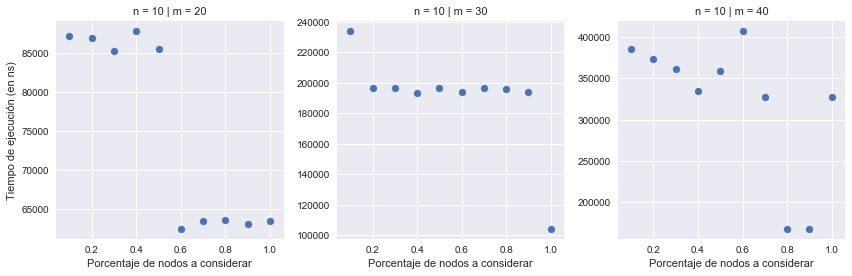
\includegraphics[scale=0.6]{img/grasp-p-multi.png}
\end{center}

La variación en performance se debe en particular a 2 motivos. Por un lado, las búsquedas golosas aleatorias generan una cierta variabilidad en los resultados obtenidos, por lo que resulta difícil determinar qué corresponde a ruido y qué a un camino de decisiones distinto. Por el otro, a medida que aumentamos el porcentaje de los nodos a considerar, permitimos que ciertas instancias ``menos óptimas'' (desde una perspectiva golosa) sean utilizadas, lo cual puede llevar a decisiones no tan útiles y, por ende, cliques más pequeñas. Esto aplica en particular a los grafos con menor cantidad de aristas, ya que mientras más tenga, mayor será en general el grado los nodos, y por consiguiente siempre se considerará agregar más nodos a la clique final.

Además de experimentar con los tiempos de ejecución, decidimos analizar la influencia de ambos parámetros de entrada de la metaheurística en la precisión de los resultados obtenidos. Para esto, utilizamos un conjunto de tests de tamaño moderado, cuyas soluciones fueron obtenidas a través del algoritmo exacto. Para cada caso de prueba, probamos distintos valores para dichos parámetros y comparamos el resultado con el obtenido por fuerza bruta.

A fines prácticos, llamaremos $it$ al número de iteraciones realizadas, y $p$ al porcentaje de nodos a considerar (entre 0 y 1).

\begin{center}
    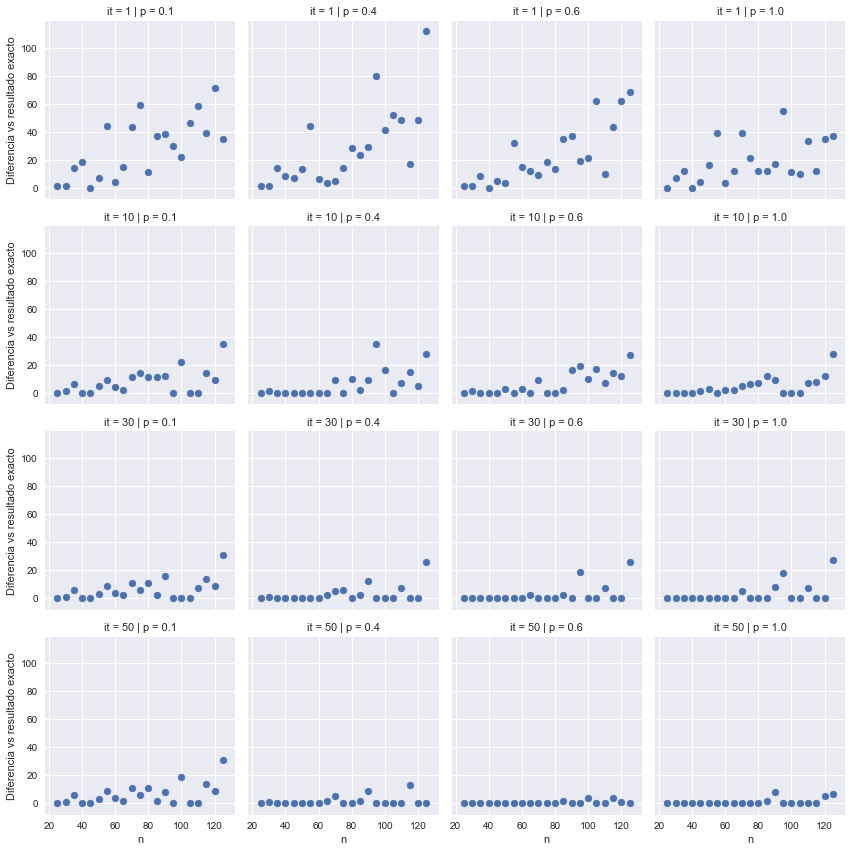
\includegraphics[scale=0.6]{img/grasp-4x4.png}
\end{center}

Este set de resultados nos resultó muy interesante. Pudimos comprobar que, casi siempre, realizar más iteraciones del algoritmo resulta en un resultado mejor (cosa que nos resultaba trivial, aunque podría no haber mejorado mucho). Por otro lado, también confirmamos que, por si solo, considerar más nodos no mejora de manera muy significativa los resultados. Sin embargo, nos tomó por sorpresa que, al realizar múltiples iteraciones ($it \geq 30$), considerar más nodos ($p \geq 0.6$) aparenta también mejorar bastante los resultados, aunque no en todas las situaciones.
 
Se debe tener en cuenta que estos resultados no son 100\% determinísticos, ya que los nodos escogidos varían de acuerdo al valor de p. Sin embargo, en base a este gráfico podemos afirmar que (para los casos de prueba utilizados) realizar aproximadamente 50 iteraciones y considerando el 60\% de los nodos de mayor grado, nuestra implementación de la metaheurística GRASP es casi tan precisa como una búsqueda por fuerza bruta.

\begin{center}
    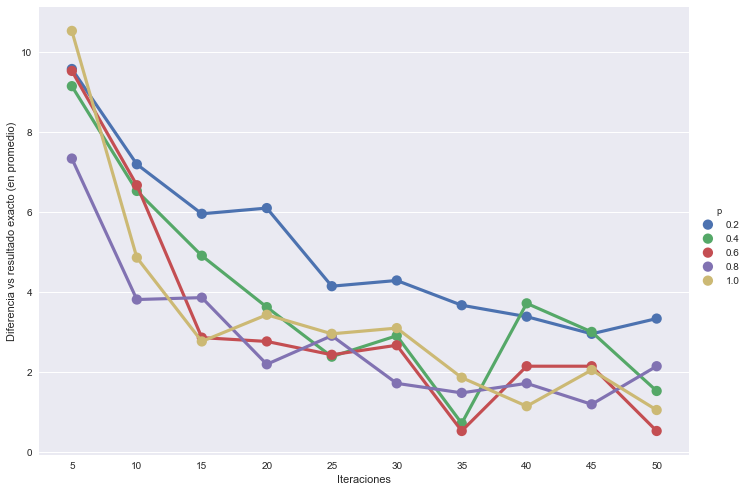
\includegraphics[scale=0.6]{img/grasp-it-v-p.png}
\end{center}

Al ver más de cerca los datos, promediando las diferencias de todos nuestros casos de prueba, podemos observar la variabilidad de nuestro algoritmo: en promedio, nuestras pruebas dieron resultados igual de precisos con $p = 0.6$ realizando 35 o 50 iteraciones. Es más, para ningún valor de p obtuvimos una linea estrictamente decreciente, que sería lo esperable de algorítmos determinísticos.

También podemos ver que en varias ocasiones, para distintas cantidades de iteraciones, otros valores de p dieron resultados más precisos. Sin embargo, consideramos que aumentar la cantidad de iteraciones reduce la variabilidad introducida por las búsquedas golosas aleatorias (porque al iterar siempre conservamos el mejor resultado), por lo que la mayor cantidad de iteraciones es más representativa del valor óptimo de p.